\chapter{Attacker Models}\label{chapter:attack-surface-models}
When discussing containers make the distinction between two perspectives: \emph{inside} a container and \emph{outside} a container.

When \emph{inside} a container, we see the container like a process that is running inside that container. That process (and thus our viewpoint) has been isolated from the host and can only see files and resources specific to that container. This means that we are able to execute commands, but only inside the container.

When \emph{outside} a container, we see the host and containers running on the host like a process that is running on the host. We are able to see everything on that host (that we have access too). For example, we are able to see the Docker daemon process and all its child processes. We are able to execute commands directly on the host. We are able to use Docker (e.g.\ interact with containers) if we have permission to use Docker (see \autoref{background:docker-socket}).

\medskip

We can think of these perspectives as attacker models. An attacker model is a general representation of a how an attacker would attack a specific system. Because we split containers into two perspectives, we see two attacker models.

We can think of the first perspective (inside a container) as an attacker model where an attacker has gained access to a container. The attacker is able to execute commands inside the container and has access to everything inside the container. Because the attacker will mostly focus on escaping the isolation that the container brings, we call this type of attack a \emph{Container Escape}. We further discuss Container Escapes in \autoref{subsection:container-escape}.

We can think of the second perspective (outside a container) as an attacker model where the attacker has unprivileged access to a host. The attacker is able to execute commands on the host, but does not have access to everything. Because the attacker will use Docker (specifically the Docker daemon) on the host to access, we call this type of attack \emph{Docker Daemon Attack}. We further discuss Daemon Attacks in \autoref{attacker-model:daemon-attacks}

Throughout this thesis we will always make the distinction between these attacker models.

\medskip

To clarify the attacker models, we will take a look at the image in \autoref{fig:attacker-model-empty} with arrows to visualize what is attacking what.

\begin{figure}[ht]
    \centering
    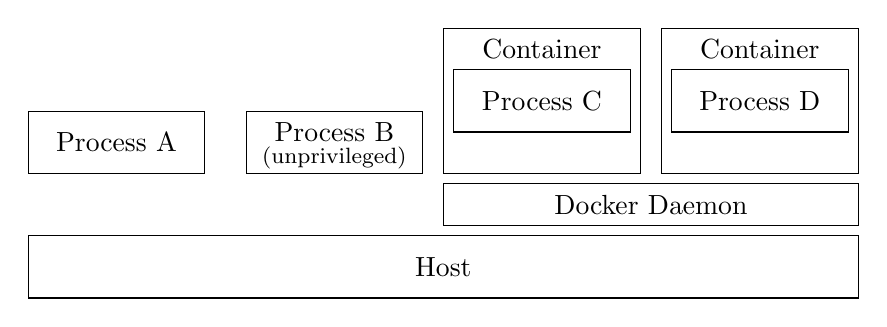
\begin{tikzpicture}[x=0.75pt,y=0.75pt,yscale=-1,xscale=1]
        % Host Rectangle
        \draw (0,100) -- (400,100) -- (400,130) -- (0,130) -- cycle ;
        \draw (200, 115) node {Host};

        %Docker Daemon Rectangle
        \draw (200,75) -- (400,75) -- (400,95) -- (200,95) -- cycle ;
        \draw (300,85) node {Docker Daemon};

        % Process A Rectangle
        \draw (0,40) -- (85,40) -- (85,70) -- (0,70) -- cycle ;
        \draw (42.5,55) node {Process A};

        % Process B Rectangle
        \draw (105,40) -- (190,40) -- (190,70) -- (105,70) -- cycle ;
        \draw (147.5,50) node {Process B};
        \draw (147.5,62.5) node {{\footnotesize (unprivileged)}};

        %Container Process C Rectangle
        \draw (200,0) -- (295,0) -- (295,70) -- (200,70) -- cycle ;
        \draw (247.5,10) node {Container};

        %% Process C Rectangle
        \draw (205,20) -- (290,20) -- (290,50) -- (205,50) -- cycle ;
        \draw (247.5,35) node {Process C};

        %Container Process D Rectangle
        \draw (305,0) -- (400,0) -- (400,70) -- (305,70) -- cycle ;
        \draw (352.5,10) node {Container};

        %% Process D Rectangle
        \draw (310,20) -- (395,20) -- (395,50) -- (310,50) -- cycle ;
        \draw (352.5,35) node {Process D};

    \end{tikzpicture}
    \caption{}\label{fig:attacker-model-empty}
    \medskip
    \small
    Two processes running directly on a host and two processes running inside Docker containers.
\end{figure}

We see the following processes pictured in the images:
\begin{enumerate}[A.]
    \item A standard (privileged) process running directly on the host.
    \item A standard unprivileged process running directly on the host.
    \item A process running in a Docker container.
    \item Similar to C.
\end{enumerate}

\section{Container Escapes}\label{subsection:container-escape}
In a container escape, an attacker has gained access to a container and tries to escape its isolation. When an attacker gains access to a container, they have gained a foothold inside their target, but that foothold is (like everything else inside the container) isolated from the host. Container escapes focus on attacking and bypassing the isolation and protection mechanics that separate the container from the host and other containers.

\medskip

\begin{figure}[ht]
    \centering
    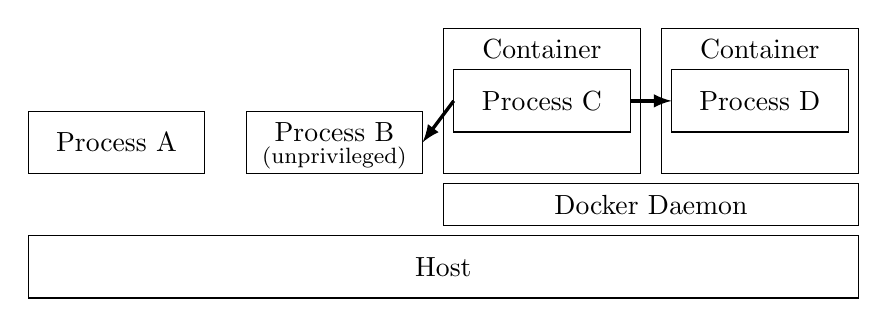
\begin{tikzpicture}[x=0.75pt,y=0.75pt,yscale=-1,xscale=1]
        % Host Rectangle
        \draw (0,100) -- (400,100) -- (400,130) -- (0,130) -- cycle ;
        \draw (200, 115) node {Host};

        %Docker Daemon Rectangle
        \draw (200,75) -- (400,75) -- (400,95) -- (200,95) -- cycle ;
        \draw (300,85) node {Docker Daemon};

        % Process A Rectangle
        \draw (0,40) -- (85,40) -- (85,70) -- (0,70) -- cycle ;
        \draw (42.5,55) node {Process A};

        % Process B Rectangle
        \draw (105,40) -- (190,40) -- (190,70) -- (105,70) -- cycle ;
        \draw (147.5,50) node {Process B};
        \draw (147.5,62.5) node {{\footnotesize (unprivileged)}};

        %Container Process C Rectangle
        \draw (200,0) -- (295,0) -- (295,70) -- (200,70) -- cycle ;
        \draw (247.5,10) node {Container};

        %% Process C Rectangle
        \draw (205,20) -- (290,20) -- (290,50) -- (205,50) -- cycle ;
        \draw (247.5,35) node {Process C};

        %Container Process D Rectangle
        \draw (305,0) -- (400,0) -- (400,70) -- (305,70) -- cycle ;
        \draw (352.5,10) node {Container};

        %% Process D Rectangle
        \draw (310,20) -- (395,20) -- (395,50) -- (310,50) -- cycle ;
        \draw (352.5,35) node {Process D};

        % Lines
        \draw [latex-,very thick] (190,55) -- (205,35) ;
        \draw [-latex, very thick] (290,35) -- (310,35) ;
    \end{tikzpicture}
    \caption{}\label{fig:container-escape}
    \medskip
    \small
    A process (Process C) running inside a container accessing data on the host (that it should not be able to access), in this case Process B.
\end{figure}

In \autoref{fig:container-escape} we see two variants of container escapes. We see Process C accessing Process B, which is a process that runs directly on the host. We also see Process C accessing Process D, which is inside another container. In both cases Process C escapes the isolation of the container and accesses data that it should not have access too.

In the first variant, Process C escapes the container to access data that it should not have access to on the host.

In the second variant, Process C escapes from its container and accesses another container. Containers should not only be isolated from the host, but also from other containers. This allows multiple containers with sensitive data to be run on the same host without them being able to access each other's data.

\medskip

An example attack scenario would be a company that offers Platform as a Service (PaaS) products that allows customers to run Docker containers on their infrastructure.\footnote{This is quite common nowadays. All major computing providers offer such a service.} If it is possible for the attacker to submit a Docker image with a malicious process that escapes the container and access the underlying infrastructure, they could access other containers or other internal resources. That would, obviously, be a big problem for the company.

\medskip

It should be noted that an exploit that allows someone to escape from a Linux \lstinline{namespace} is essentially a container escape exploit, because Docker relies heavily on \lstinline{namespaces} for isolation (see \autoref{subsubsection:internals}). CVE--2017--7308~\cite{CVE-2017-7308} is a good example of this.

\section{Docker Daemon Attacks}\label{attacker-model:daemon-attacks}
In a Docker daemon attack, an attacker has access to a host with Docker installed on it. The attacker might be able access sensitive and privileged information by interacting with the Docker daemon or by reading Docker configuration files. Unlike container escapes, the attacker does not attack Docker or the isolation that Docker creates directly, but uses Docker to perform malicious actions.

\medskip

This is attack is shown in \autoref{fig:docker-daemon-attack}.

\begin{figure}[ht]
    \centering
    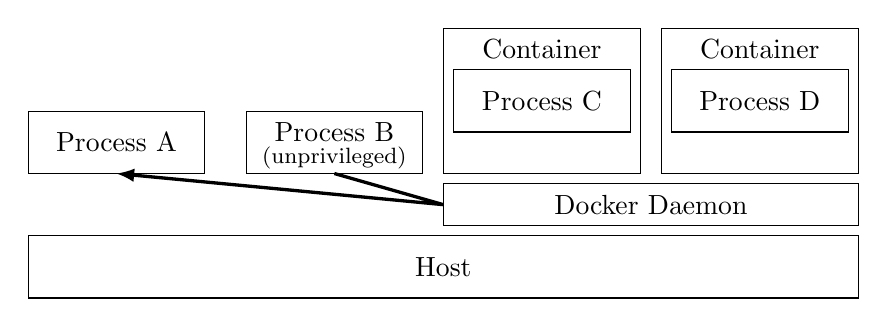
\begin{tikzpicture}[x=0.75pt,y=0.75pt,yscale=-1,xscale=1]
        % Host Rectangle
        \draw (0,100) -- (400,100) -- (400,130) -- (0,130) -- cycle ;
        \draw (200, 115) node {Host};

        %Docker Daemon Rectangle
        \draw (200,75) -- (400,75) -- (400,95) -- (200,95) -- cycle ;
        \draw (300,85) node {Docker Daemon};

        % Process A Rectangle
        \draw (0,40) -- (85,40) -- (85,70) -- (0,70) -- cycle ;
        \draw (42.5,55) node {Process A};

        % Process B Rectangle
        \draw (105,40) -- (190,40) -- (190,70) -- (105,70) -- cycle ;
        \draw (147.5,50) node {Process B};
        \draw (147.5,62.5) node {{\footnotesize (unprivileged)}};

        %Container Process C Rectangle
        \draw (200,0) -- (295,0) -- (295,70) -- (200,70) -- cycle ;
        \draw (247.5,10) node {Container};

        %% Process C Rectangle
        \draw (205,20) -- (290,20) -- (290,50) -- (205,50) -- cycle ;
        \draw (247.5,35) node {Process C};

        %Container Process D Rectangle
        \draw (305,0) -- (400,0) -- (400,70) -- (305,70) -- cycle ;
        \draw (352.5,10) node {Container};

        %% Process D Rectangle
        \draw (310,20) -- (395,20) -- (395,50) -- (310,50) -- cycle ;
        \draw (352.5,35) node {Process D};

        % Line
        \draw [-latex, very thick] (147.5,70) -- (200,85) -- (42.5,70);
    \end{tikzpicture}
    \caption{}\label{fig:docker-daemon-attack}
    \medskip
    \small
    An unprivileged process B accessing privileged data (in the image process A) using the Docker daemon.
\end{figure}

Because Docker needs a lot of kernel features to function properly, the Docker daemon needs to run as \lstinline{root}. This makes it a very interesting target, because vulnerabilities that allow an attacker to maliciously control the Docker daemon, allow the attacker to perform actions as \lstinline{root}.

